\documentclass[tikz,border=5pt]{standalone}
\usepackage{tikz}
\usetikzlibrary{positioning, arrows.meta, calc, fit, backgrounds}

\begin{document}
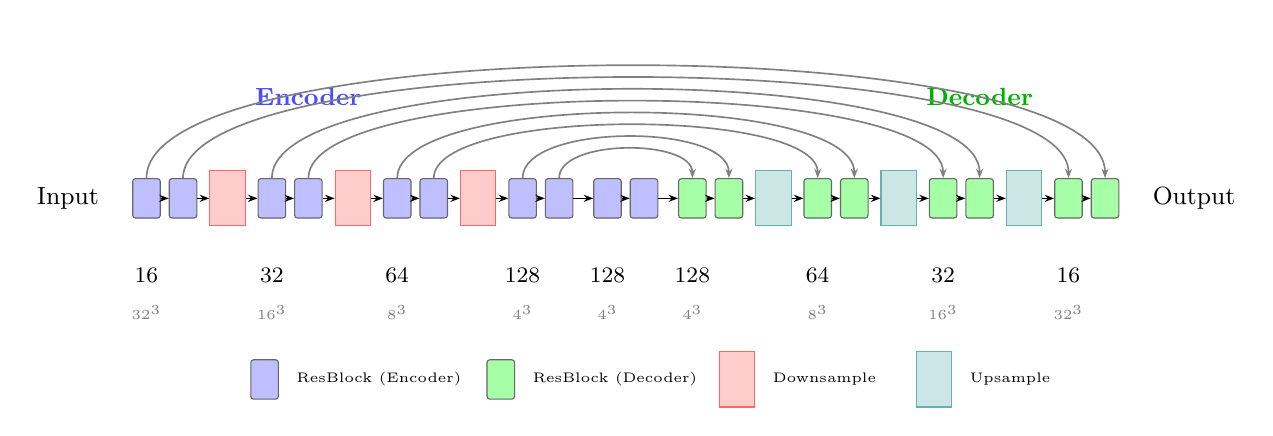
\begin{tikzpicture}[
    res/.style={rectangle, draw=black!60, fill=#1, minimum width=0.35cm, minimum height=0.5cm, rounded corners=1pt, font=\tiny},
    down/.style={rectangle, draw=red!60, fill=red!20, minimum width=0.45cm, minimum height=0.7cm, font=\tiny},
    up/.style={rectangle, draw=teal!60, fill=teal!20, minimum width=0.45cm, minimum height=0.7cm, font=\tiny},
    arrow/.style={-{Stealth[length=1.2mm]}, semithick},
    skip/.style={-{Stealth[length=1.2mm]}, gray, semithick},
]

% ========== ENCODER ==========
% Level 1 (channels=16)
\node[res=blue!25] (r1a) at (0, 0) {};
\node[res=blue!25, right=0.1cm of r1a] (r1b) {};
\node[down, right=0.15cm of r1b] (d1) {};

% Level 2 (channels=32)
\node[res=blue!25, right=0.15cm of d1] (r2a) {};
\node[res=blue!25, right=0.1cm of r2a] (r2b) {};
\node[down, right=0.15cm of r2b] (d2) {};

% Level 3 (channels=64)
\node[res=blue!25, right=0.15cm of d2] (r3a) {};
\node[res=blue!25, right=0.1cm of r3a] (r3b) {};
\node[down, right=0.15cm of r3b] (d3) {};

% Level 4 (channels=128)
\node[res=blue!25, right=0.15cm of d3] (r4a) {};
\node[res=blue!25, right=0.1cm of r4a] (r4b) {};

% ========== MIDDLE ==========
\node[res=blue!25, right=0.25cm of r4b] (m1) {};
\node[res=blue!25, right=0.1cm of m1] (m2) {};

% ========== DECODER ==========
% Level 4 (channels=128→64)
\node[res=green!35, right=0.25cm of m2] (t4a) {};
\node[res=green!35, right=0.1cm of t4a] (t4b) {};
\node[up, right=0.15cm of t4b] (u3) {};

% Level 3 (channels=64→32)
\node[res=green!35, right=0.15cm of u3] (t3a) {};
\node[res=green!35, right=0.1cm of t3a] (t3b) {};
\node[up, right=0.15cm of t3b] (u2) {};

% Level 2 (channels=32→16)
\node[res=green!35, right=0.15cm of u2] (t2a) {};
\node[res=green!35, right=0.1cm of t2a] (t2b) {};
\node[up, right=0.15cm of t2b] (u1) {};

% Level 1 (channels=16)
\node[res=green!35, right=0.15cm of u1] (t1a) {};
\node[res=green!35, right=0.1cm of t1a] (t1b) {};

% ========== LABELS ==========
% Input/Output
\node[left=0.3cm of r1a, font=\small] {Input};
\node[right=0.3cm of t1b, font=\small] {Output};

% Channel numbers below
\node[below=0.5cm of r1a, font=\footnotesize] (c1) {16};
\node[below=0.5cm of r2a, font=\footnotesize] (c2) {32};
\node[below=0.5cm of r3a, font=\footnotesize] (c3) {64};
\node[below=0.5cm of r4a, font=\footnotesize] (c4) {128};
\node[below=0.5cm of m1, font=\footnotesize] (cm) {128};
\node[below=0.5cm of t4a, font=\footnotesize] (c4d) {128};
\node[below=0.5cm of t3a, font=\footnotesize] (c3d) {64};
\node[below=0.5cm of t2a, font=\footnotesize] (c2d) {32};
\node[below=0.5cm of t1a, font=\footnotesize] (c1d) {16};

% Resolution below channels
\node[below=0.05cm of c1, font=\tiny, gray] {$32^3$};
\node[below=0.05cm of c2, font=\tiny, gray] {$16^3$};
\node[below=0.05cm of c3, font=\tiny, gray] {$8^3$};
\node[below=0.05cm of c4, font=\tiny, gray] {$4^3$};
\node[below=0.05cm of cm, font=\tiny, gray] {$4^3$};
\node[below=0.05cm of c4d, font=\tiny, gray] {$4^3$};
\node[below=0.05cm of c3d, font=\tiny, gray] {$8^3$};
\node[below=0.05cm of c2d, font=\tiny, gray] {$16^3$};
\node[below=0.05cm of c1d, font=\tiny, gray] {$32^3$};

% Section labels above
\node[above=0.8cm of r2b, font=\small\bfseries, blue!70] {Encoder};
\node[above=0.8cm of t2b, font=\small\bfseries, green!70!black] {Decoder};

% ========== ARROWS (data flow) ==========
\draw[arrow] (r1a) -- (r1b);
\draw[arrow] (r1b) -- (d1);
\draw[arrow] (d1) -- (r2a);
\draw[arrow] (r2a) -- (r2b);
\draw[arrow] (r2b) -- (d2);
\draw[arrow] (d2) -- (r3a);
\draw[arrow] (r3a) -- (r3b);
\draw[arrow] (r3b) -- (d3);
\draw[arrow] (d3) -- (r4a);
\draw[arrow] (r4a) -- (r4b);
\draw[arrow] (r4b) -- (m1);
\draw[arrow] (m1) -- (m2);
\draw[arrow] (m2) -- (t4a);
\draw[arrow] (t4a) -- (t4b);
\draw[arrow] (t4b) -- (u3);
\draw[arrow] (u3) -- (t3a);
\draw[arrow] (t3a) -- (t3b);
\draw[arrow] (t3b) -- (u2);
\draw[arrow] (u2) -- (t2a);
\draw[arrow] (t2a) -- (t2b);
\draw[arrow] (t2b) -- (u1);
\draw[arrow] (u1) -- (t1a);
\draw[arrow] (t1a) -- (t1b);

% ========== SKIP CONNECTIONS ==========
\draw[skip] (r4b.north) .. controls ++(0, 0.5) and ++(0, 0.5) .. (t4a.north);
\draw[skip] (r4a.north) .. controls ++(0, 0.7) and ++(0, 0.7) .. (t4b.north);

\draw[skip] (r3b.north) .. controls ++(0, 0.9) and ++(0, 0.9) .. (t3a.north);
\draw[skip] (r3a.north) .. controls ++(0, 1.1) and ++(0, 1.1) .. (t3b.north);

\draw[skip] (r2b.north) .. controls ++(0, 1.3) and ++(0, 1.3) .. (t2a.north);
\draw[skip] (r2a.north) .. controls ++(0, 1.5) and ++(0, 1.5) .. (t2b.north);

\draw[skip] (r1b.north) .. controls ++(0, 1.7) and ++(0, 1.7) .. (t1a.north);
\draw[skip] (r1a.north) .. controls ++(0, 1.9) and ++(0, 1.9) .. (t1b.north);

% ========== LEGEND (centered) ==========
\begin{scope}[shift={(6, -2.3)}]
    \node[res=blue!25, minimum width=0.35cm, minimum height=0.5cm] (leg1) at (-4.5, 0) {};
    \node[right=0.1cm of leg1, font=\tiny] {ResBlock (Encoder)};
    
    \node[res=green!35, minimum width=0.35cm, minimum height=0.5cm] (leg2) at (-1.5, 0) {};
    \node[right=0.1cm of leg2, font=\tiny] {ResBlock (Decoder)};
    
    \node[down, minimum width=0.45cm, minimum height=0.7cm] (leg3) at (1.5, 0) {};
    \node[right=0.1cm of leg3, font=\tiny] {Downsample};
    
    \node[up, minimum width=0.45cm, minimum height=0.7cm] (leg4) at (4, 0) {};
    \node[right=0.1cm of leg4, font=\tiny] {Upsample};
\end{scope}

\end{tikzpicture}
\end{document}
